%
% introduction.tex
%
% Copyright (C) 2021 by SpaceLab.
%
% Battery Module 4C Documentation
%
% This work is licensed under the Creative Commons Attribution-ShareAlike 4.0
% International License. To view a copy of this license,
% visit http://creativecommons.org/licenses/by-sa/4.0/.
%

%
% \brief Introduction chapter.
%
% \author Gabriel Mariano Marcelino <gabriel.mm8@gmail.com>
% \author André Martins Pio de Mattos <andrempmattos@gmail.com>
% \author Yan Castro de Azeredo <yan.ufsceel@gmail.com>
%
% \institution Universidade Federal de Santa Catarina (UFSC)
%
% \version 0.1.1
%
% \date 2020/01/21
%

\chapter{Introduction} \label{ch:introduction}

The {Battery Module 4C}\nomenclature{\textbf{BATC4}}{\textit{Battery Module 4C.}} is a separate board from the EPS2\nomenclature{\textbf{EPS}}{\textit{Energy Power System.}} \cite{eps2} in order to accommodate 4 lithium-ion cells. Besides the cells, the board has connectors for interfacing signals and power lines with the EPS2 module, 2 power resistors to operate as heaters to maintain the cells temperature during eclipse periods, and 4 temperature sensors. The batteries used are the \textbf{ICR18650-30B} lithium-ion cells, which are connected in series and parallel to supply the required voltage and current. Each cell is fixed with \textbf{18650} metal holders and between the pairs there is the power resistor attached with a thermal element in the middle. A mechanical mount is placed over the batteries and screwed to the board, providing better stress resistance. Also, there are PC104 through hole pads present on the board for a connector that could be used for making mechanical integration with the EPS, or with future improvements a interface for power, data or control signals.

The board is a direct improvement from the first battery board used in the FloripaSat-1 mission \cite{battery-board-1}. All the project, source and documentation files are available freely on a GitHub repository \cite{bat4c} under its repectives licenses.

\begin{figure}[!ht]
    \begin{center}
        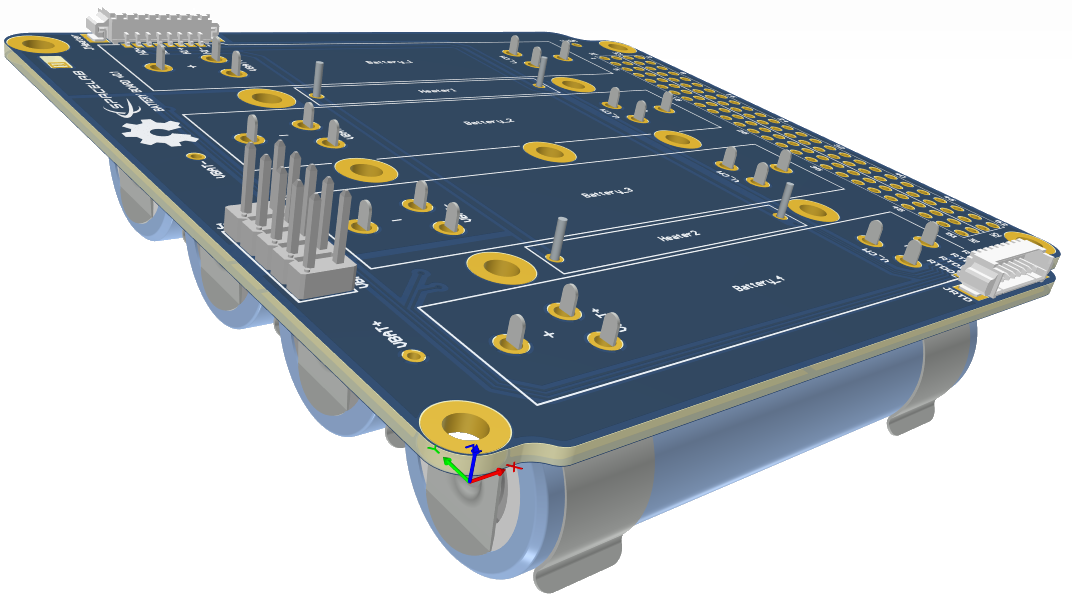
\includegraphics[width=0.65\textwidth]{figures/bat4c-pcb-3d.png}
        \caption{3D view of the Battery Module 4C PCB.}
        \label{fig:pcb-3d}
    \end{center}
\end{figure}